
\chapter{Background}\label{section:background}

\section{Information Retrieval (IR) and Search Engine}\label{section:IR}
``Information Retrieval (IR) is the activity of obtaining information resources relevant to an information need from a collection of information resources''~\cite{IR}. 
An information retrieval process begins when a user 
enters a query into the system. Queries are formal statements of information needs, for example search strings in web search engines. However, the 
submitted query may not give the satisfying results for the user. In this case, the process begins again. Figure~\ref{fig:retrieval_process} illustrates
search process. As information resources were not originally intended for access (Retrieval of unstructured data)[P. 7]~\cite{IRlecture}, 
it is impossible for a user query to uniquely identify a single object in the collection. Instead, several objects may match the query, 
with different degrees of relevancy. In IR field, there are various types of retrieval models used to compute the degree of relevancy. This will
be discussed in more details in section~\ref{section:retrieving}.

A search engine is an information retrieval system designed to help find information stored on a computer system~\cite{searchengine}. The search results are usually 
presented in a list ordered by the degree of relevancy and are commonly called hits. 
Search engines help to minimize the time required to find information and the amount of 
information which must be consulted~\cite{searchengine}. The special kind of search engine is 
web search engine. It is a software system that is designed to search for information on the World Wide Web~\cite{websearchengine} such as Google, 
Bing, and Yahoo.

\begin{figure}
\centering
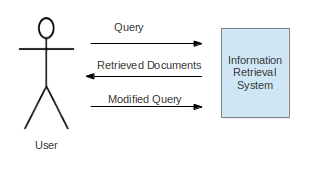
\includegraphics[scale=1]{./figures/retrieval_process.png}
\caption{Search Process} \label{fig:retrieval_process}
\end{figure}

\subsection{Brief Overview of Information Retrieval System Architecture}\label{section:IRarchitecture}
In IR systems, two main objectives have to be met~\cite{IRarchitecture} - first, the results must satisfy user - this means retrieving information to meet user's
information need. Second, retrieving process must be fast. This section is devoted to a brief overiew of the architecture of IR systems 
which is very important to meet IR main objectives. It also explains readers
how documents are retrieved and the data structure used in IR systems. To understand how retrieval process works, we must understand 
indexing process first. This process is performed offline and only one time. 
There are 4 steps involved in indexing process and each process is performed sequentially~\cite{IRarchitecture}:
\begin{enumerate}
 \item Tokenisation
 \item Stopwords Removal
 \item Stemming
 \item Inverted Index Structure Creation
\end{enumerate}

Given a document containing Albert Einstein's quote about life, it can be illustrated in a terms-frequency table.

\begin{quotation}
 \item \textit{There are only two ways to live your life. One is as though nothing is a miracle. The other is as though everything is a miracle.}
\end{quotation}


\begin{figure}
\centering
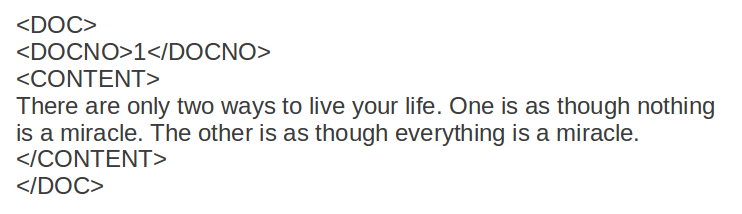
\includegraphics[scale=0.5]{./figures/text.png}
\caption{Document} \label{fig:quote} 
\end{figure}

\begin{table}
\centering
\begin{tabular}{|c|c|}

\hline \textbf{Term} & \textbf{frequency} \\
\hline there & 1 \\
\hline are & 1 \\
\hline only & 1 \\ 
\hline two & 1 \\
\hline ways & 1 \\
\hline live & 1 \\
\hline your & 1 \\
\hline life & 1 \\
\hline to & 1 \\
\hline one & 1 \\
\hline is & 3 \\
\hline as & 2 \\
\hline though & 2 \\
\hline nothing & 1 \\
\hline a & 2 \\
\hline miracle & 2 \\
\hline the & 1 \\
\hline other & 1 \\
\hline everything & 1 \\  
\hline
\end{tabular}
\caption{Terms and Frequency} \label{table:termsandfrequency}
\end{table}

Table \ref{table:termsandfrequency} shows all the terms and frequency of each term in the document. It can be seen that there are some words in the 
document which occur too frequently. These words are not good discriminators. They are referred to as ``stopwords''. Stopwords include
articles, prepositions, and conjunctions etc.

\paragraph{Tokenisation}
is the process of breaking a stream of text into words called tokens(terms)~\cite{tokenization}. The stream of text will be used by other indexing processes.

\paragraph{Stopwords Removal}
is the process of removing stopwords in order to reduce the size of the indexing structure~\cite[P. 15]{IRarchitecture}.
Table \ref{table:stopwordsremoval} shows all the terms and frequency of each term after stopwords removal process.

\begin{table}
\centering
\begin{tabular}{|c|c|}
\hline \textbf{Term} & \textbf{frequency} \\
\hline two & 1 \\
\hline ways & 1 \\
\hline live & 1 \\
\hline life & 1 \\
\hline one & 1 \\
\hline nothing & 1 \\
\hline miracle & 2 \\
\hline everything & 1 \\  
\hline
\end{tabular}
\caption{Terms and Frequency After Stopwords Removal} \label{table:stopwordsremoval}
\end{table}
%Now, the table representing the document has shorter size and contains only meaningful words.

\paragraph{Stemming} is the process of reducing all words obtained with the same root into a single root~\cite[P. 20]{IRarchitecture}. 
A stem is the portion of a word which is left after
the removal of its affixes (i.e. prefixes and suffixes). For example, connect is the stem for the variants connected, connecting, and connection.
This process makes the size of the data shorter. There are various stemming algorithms such as Porter Stemming, and Suffix-stripping algorithms.

\begin{table}
\centering
\begin{tabular}{|c|c|}
\hline \textbf{Term} & \textbf{frequency} \\
\hline two & 1 \\
\hline way & 1 \\
\hline live & 1 \\
\hline life & 1 \\
\hline one & 1 \\
\hline nothing & 1 \\
\hline miracle & 2 \\
\hline everything & 1 \\  
\hline
\end{tabular}
\caption{Terms and Frequency After Stemming} \label{table:stemming}
\end{table}
After stemming, all terms in the table are in its root forms. If a document is large in size, this process can reduce the size of the data considerably. However, 
there is one drawback. That is, it prevents interpretation of word meanings. For instance, the root form of the term ``gravitation'' is ``gravity''. But
the meaning of ``gravitation'' is different from ``gravity''.

\begin{figure}
\centering
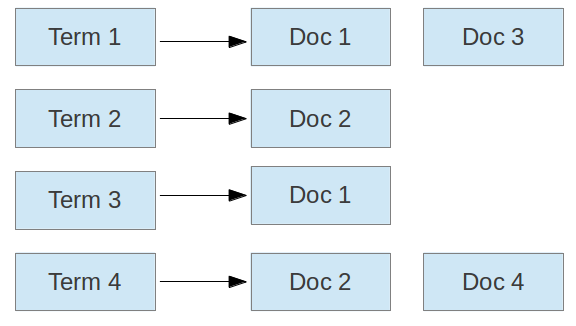
\includegraphics[scale=0.5]{./figures/invertedIndex.png}
\caption{Simple Inverted Index} \label{fig:invertedIndex} 
\end{figure}

\paragraph{Inverted Index Structure Creation} is the process that creates an index data structure storing a mapping from terms(keys) to its 
locations in a database file, or in a document or a set of documents(values)~\cite{invertedindex}. 
The purpose of this data structure is to allow a full text searches. In IR, a value in a key-value pair is called posting. There are a number of index
structures used in practice. However, the index used in most IR systems and in this project is inverted index.
Figure \ref{fig:invertedIndex} shows a simple inverted index. Given a query (a set of terms), it is now possible to efficiently search for
documents containing those terms. However, each posting may contain additional information or features
about a document such as the freqency of the term etc.

\subsection{Retrieval Models}\label{section:retrievalmodel}
In the previous section, basic indexing process was briefly explained. In this section, we will give a brief introduction to a few retrieval models including one
used in this project. In general, retrieval models can be categorised into 2 categories: probabilistic approach and non probabilistic approach.
This section will briefly explain Term Frequency–Inverse Document Frequency (tf-idf), BM25 and PL2 retrieval models.

\paragraph{Term Frequency–Inverse Document Frequency (tf-idf)} \hspace{0pt} \\
\indent tf-idf is a numerical statistic that is intended to reflect how important a word is to a document in a collection~\cite{tfidf}. As the name suggests, it consists
of 2 parts: term frequency (tf) and inverse document frequency (idf). Term frequency is the number of occurrences a term appears in a document.
Inverse document frequency (idf) is a measure of whether the term is common or rare across all documents~\cite{tfidf}.
This component is very important for instance, if a query term appears in most of the documents in the corpus, it is not appropriate to give a 
document containing that term a high score because that term is not a very good discriminator. On the other hand, it is appropriate to give high scores to 
documents containing terms rarely apprear in the corpus.
The following is the formula of \textbf{tf-idf} weighting model:
\begin{equation}
W_{fk} = f_{fd}log \frac{N + 1}{D_k + 1}
\end{equation}
where $N$ is the number of documents in the collection, $f_{fd}$ is tf of ${k^{th}}$ keyword in document $d$ (term frequency),
and $D_k$ is the number of documents containing ${k^{th}}$ keyword. The $log \frac{N + 1}{D_k + 1}$ is the idf of the model.
The numerator and denominator are added by 1 to prevent possibility of zero.
This model is a non-probabiltic approach and is one of the easiest to implement models in IR.

\paragraph{BM25} \hspace{0pt} \\
BM25 is a very popular probabiltic retrieval model in IR. Why use probabilities? 
In section~\ref{section:IR}, we explained that IR deals with uncertain and unstructured information. In other words, we do not know specifically
what the documents are really about. As a consequence, a query does not uniquely identify a single object in the collection. Therefore, probability theory
seems to be the most natural way to quantify uncertainty~\cite[P. 7]{probModel}.

%Let $x$ be a document in the collection, $R_{d\vec{q}}$ represent the \textit{relevance} of a document $d$ with respect to query $\vec{q}$. 

\begin{equation}\label{eq:BM25}
\sum_{t \in \vec{q}} log_2 \frac{r_t/(R - r_t)}{(n_t - r_t)/(N - n_t - R + r_t)} \frac{(k_1 + 1)\cdot tf_{td}}{K + tf_{td}} \frac{k_2 + 1)\cdot tf_{tq}}{k_2 + tf_{tq}}
\end{equation}
where $K$ = $k_t((1 - b) + b\frac{dl}{avdl})$, $tf_tq$ and $tf_td$ are the frequency of term $t$ in the query $\vec{q}$ and document $d$ respectively,
and $b$, $dl$ and $avdl$ are paraameters set empirically. The proof of BM25 is beyond the scope of the project.

\paragraph{PL2} \hspace{0pt} \\
PL2 is a model from the divergence from randomness framework, based on a poisson distribution~\cite{craig}. This project uses PL2 weight model to 
calculate document scores. This model is also a probabilistic approach. Given a document $d$ and a query $\vec{q}$, the formula of PL2~\cite[P. 23-24]{craigthesis} is given below:

\begin{equation}\label{eq:pl2}
 score(d, \vec{q}) = \sum_{t \in \vec{q}} qtw\cdot \frac{1}{tfn + 1}(tfn\cdot log_2\frac{tfn}{\lambda} + 
 (\lambda - tfn)\cdot log_2e + 0.5\cdot log_2(2\pi \cdot tfn))
\end{equation}
where $\lambda$ is the mean and variance of a Poisson distribution, and the query weight term $qtw$ is given by $qtf/qtf_{max}$.
$qtf$ is the query term frequency. $qtf_{max}$ is the maximum query term frequency among the query terms. From equation~\ref{eq:pl2}, 
\[tfn = tf\cdot log_2(1 + c\cdot \frac{avgl}{l}), c > 0\]
where $tf$ is the actual term frequency of the term $t$ in document $d$ and $l$ is the length of the
document in tokens. $avgl$ is the average document length in the whole collection.
$c$ is the hyper-parameter that controls the normalisation applied to the term frequency
with respect to the document length.
The proof and explanation are out of the scope of the project.


\subsection{Retrieval Process in Information Retrieval}\label{section:retrieving}
\begin{figure}
\centering
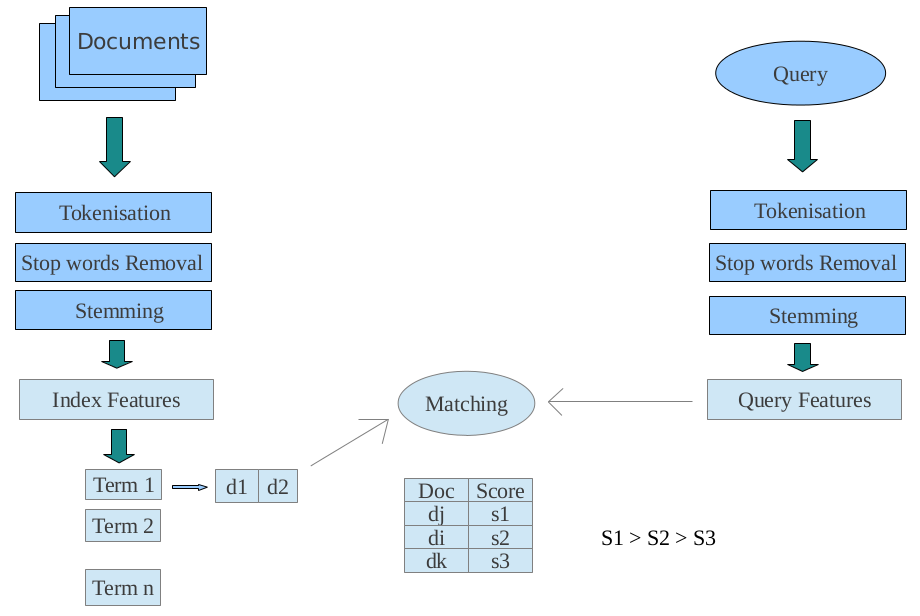
\includegraphics[scale=0.3]{./figures/retrieval.png}
\caption{Retrieval Process} \label{fig:retrieval} 
\end{figure}
Section~\ref{section:IRarchitecture} and Section~\ref{section:retrievalmodel} explained basic indexing process and a few retrieval models respectively.
In this section, we will see how documents are retrieved. Figure ~\ref{fig:retrieval} shows
retrieval process of IR system. In IR, there are 2 phases in general:
online and offline phases. The offline phase is the phase that all documents in the corpus are indexed, all features are extracted 
(section~\ref{section:IRarchitecture}) and index structure is built. 

%Then for each document, features are extracted. The feature extracting
%process is not mandatory and application dependent. One most extracted feature is the frequency of the terms occured in a document.
%This feature can be applied to both tf-idf and BM25 explained in section~\ref{section:retrievalmodel}.
%Subsequently, inverted index is built.

On the other hand, online phase begins after a user submits a query into the system. After that, tokenisation, stopwords removal and stemming processes 
are performed as same as the offline phase.
Features can also be extracted from query terms as well. At this point, it comes to the process of matching and assigning scores to documents.
This process can make use of one of the retrieval models explained in section~\ref{section:retrievalmodel}. In this project, PL2 weighting model and voting
technique which will be explained in section~\ref{section:voting} are used to compute scores.
Once scores have been assigned to relevant documents, the system ranks all documents in order of decreasing scores and 
show to the user. Figure~\ref{fig:retrieval} gives a graphical representation of retrieval process.

\subsection{Evaluation}\label{sec:evaluation}
This section is devoted to backgrounds of evaluation of IR systems. It is very important as it is a background for Evaluation Section. 
Since IR is research-based, understanding how evaluation is carried out will enable readers to determine whether 
this project is achieved or not. There are 3 main reasons for evaluating IR systems~\cite[P. 3]{eval}: 
\begin{enumerate}
 \item Economic reasons: If people are going to buy the technology, they want to know how effective it is.
 \item Scientific reasons: Researchers want to know if progress is being made. So they need a measure for progress. 
	This can show that their IR system is better or worse than someone else's.
 \item Verification: If an IR system is built, it is necessary to verify the performance.
\end{enumerate}

To measure information retrieval effectiveness in the standard way, a test collection is required and it consists of 3 things~\cite{evalweb}:
\begin{enumerate}
 \item A document collection.
 \item A test suite of information needs, expressible as queries.
 \item A set of relevance judgments, standardly a binary assessment of either relevant or nonrelevant for each query-document pair.
\end{enumerate}

The standard approach to information retrieval system evaluation revolves around the notion of relevant and nonrelevant documents. With respect 
to a user's information need, a document in the test collection is given a binary classification as either relevant or nonrelevant~\cite{evalweb}. However,
this can be extended by using numbers as an indicator of the degree of relevancy called \textbf{graded relevance value}. For example, documents labelled 2 is more relevant than documents
labelled 1, and documents labelled 0 is not relevant. There are a number of test collection stardards. In this project, Text Retrieval Conference (TREC)
is used since it is widely used in the field of IR.

%\paragraph{Precision and Recall}
\subsubsection{Precision and Recall}
The function of an IR system is to~\cite[P. 10]{eval}:
\begin{itemize}
 \item retrieve all \textit{relevant documents} measured by \textbf{Recall}
 \item retrieve \textit{no non-relevant documents} measured by \textbf{Precision}
\end{itemize}

Precision (P) is the fraction of retrieved documents that are relevant 
\begin{center}
 \raisebox{-\totalheight}{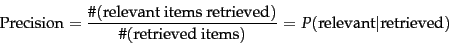
\includegraphics[scale=0.5]{./figures/precision.png}}
\end{center}

Recall (R) is the fraction of relevant documents that are retrieved 
\begin{center}
\raisebox{-\totalheight}{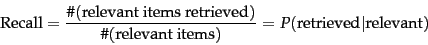
\includegraphics[scale=0.5]{./figures/recall.png}}
\end{center}

If a system has high precision but low recall, the system returns relevant documents but misses many useful ones.
If a system has low precision but high recall, the system returns most relevant documents but includes lots of junks.
Therefore, the ideal is to have both high precision and recall. To give a good example, consider Figure ~\ref{fig:pr_example}, since
overall IR system A (blue) has higher precision than IR system B (red), system A is better than system B.

\begin{figure}
\centering
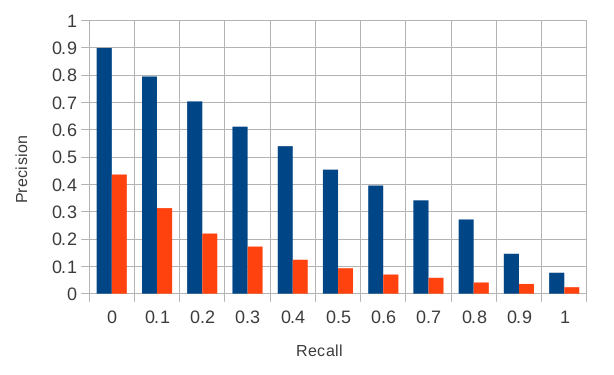
\includegraphics[scale=0.5]{./figures/pr_example.png}
\caption{Precision-Recall Graph} \label{fig:pr_example} 
\end{figure}

However, in certain cases, precisions of system A may be higher values than system B in some recall points or vice versa. Therefore,
Mean Average Precision (MAP), Normalized Discounted Cumulative Gain (NDCG) and Mean Reciprocal Rank (MRR) are used to address this problem.
Each of them has different behaviours of evaluation.

\paragraph{Mean Average Precision (MAP)} \hspace{0pt} \\
MAP for a set of queries is the mean of the average precision scores for each query~\cite{IR}. The equation below is
a formula for MAP.
\begin{center}
\raisebox{-\totalheight}{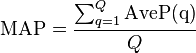
\includegraphics[scale=0.5]{./figures/map.png}}
\end{center}
where Q is the number of queries.

\paragraph{Mean Reciprocal Rank (MRR)} \hspace{0pt} \\
MRR is a statistic measure for evaluating a list of possible responses to a set of queries, ordered by 
probability of correctness~\cite{mrr}. The equation below is a formula for MRR.
\begin{center}
\raisebox{-\totalheight}{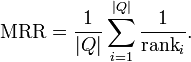
\includegraphics[scale=0.5]{./figures/mrr.png}}
\end{center}
where $rank_i$ is the position of the correct result and $|Q|$ is the number of queries.

\paragraph{Normalized Discounted Cumulative Gain (NDCG or nDCG)} \hspace{0pt} \\
To understand NDCG, first of all, we have to understand \textbf{Discounted Cumulative Gain (DCG)}. 
The premise of DCG is that highly relevant documents appearing in lower position in a search result list should be penalized as 
the graded relevance value (see last section) is 
reduced logarithmically proportional to the position of the result.~\cite{ndcg}. The discounted CG accumulated at a particular rank position
$p$ is defined as:

\begin{center}
\raisebox{-\totalheight}{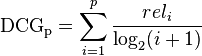
\includegraphics[scale=0.5]{./figures/dcg.png}}
\end{center}

From DCG, we can formulate NDCG as follows:
\begin{center}
\raisebox{-\totalheight}{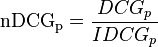
\includegraphics[scale=0.5]{./figures/ndcg.png}}
\end{center}
where $IDCG_p$ is the maximum possible (ideal) DCG for a given set of queries, documents, and relevances.


\section{Learning to Rank (LETOR)}\label{sec:letor}
Learning to rank or machine-learned ranking (MLR) is a type of supervised or semi-supervised machine learning problem in which the goal is 
to automatically construct a ranking model from training data~\cite{letor}.
Employing learning to rank techniques to learn the ranking function is important as it is viewed as
a promising approach to information retrieval~\cite{letor}. In particular, many learning to rank aproaches attempt to learn a combination of features
(called the learned model)~\cite[P. 3]{learningmodel}. The resulting learned model is applied to a vector of features for each document, to determine the final scores for 
producing the final ranking of documents for a query~\cite[P. 3]{learningmodel}.

\subsection{Query Dependent Feature}\label{section:querydependent}
Figure~\ref{fig:retrieval_process} shows a simple search process in IR. After a user submits a query into an IR system. The system ranks the results 
with respect to the query and returns a result set to the user. It can be clearly seen that the results obtained with respect to the query depends on the 
query the user submitted. In other words, document A can have 2 different degrees of relevancy if a user changes a query.
In learning to rank, this is called query dependent feature~\cite{craig}.

\subsection{Query Independent Feature}\label{section:queryindependent}
In contrast to Query Dependent Feature, a feature that does not depend on a user query is called query independent feature~\cite{craig}. This feature is fixed for each
document. For now, it is better to not dig into great details about this because this will be focused in later section.

\subsection{Learning to Rank (LETOR) File Format}\label{sec:letorFile}
From the previous 2 sections, we now know what query dependent and query independent features are. In this section, we will talk about how these features
are formatted in a file called \textbf{LETOR file}. The LETOR file is then learned to obtain a model file (see next section).
The following is the format of LETOR file:

\begin{quotation}
\noindent\#feature\_num1:feature\_name1 \\
\#feature\_num2:feature\_name2 \\
graded\_relevance\_value qid:query feature\_num1:feature\_name1\_score feature\_num2:feature\_name2\_score \#docno = document\_id
\end{quotation}

In this LETOR file, there are 2 features, \textit{feature\_name1} and \textit{feature\_name2}. In LETOR file, items after a hash key are ignored.
The lines not preceded by hash key are learned. They represent documents with scores
of each feature. \textit{graded\_relevance\_value} is a label which indicates the degree of relevancy (see last section).
If the label is 0, it means the document is irrelevant with respect to a query. If it is 1, the document is relevant. 
In this project, \textit{graded\_relevance\_value} range from 0 to 2 in order of 
the degree of relevancy. To the left of the label is a \textit{query} preceded by \textit{$qid:$} and scores of each feature associated to a document.
There can be any number of documents in the LETOR file.

\subsection{Learning to Rank (LETOR) Model File Format}
After a LETOR file is learned, we obtain a \textit{Learned Model}. This section aims to show some learned model file formats.
\begin{quotation}
\noindent \#\# Coordinate Ascent \\
\#\# Restart = 2 \\
\#\# MaxIteration = 25 \\
\#\# StepBase = 0.05 \\
\#\# StepScale = 2.0 \\
\#\# Tolerance = 0.001 \\
\#\# Regularized = false \\
\#\# Slack = 0.001 \\
1:0.64 2:4.34 3:4.3 4:2.0 5:1.2 6:9.1 7:3.3
\end{quotation}
The lines preceded are ignored. The above learned model applies \textit{Coordinate Ascent} LETOR technique. Knowing what parameters preceded by a hash key
mean is out of the scope of the project. We only take lines not preceded by a hash key into account. According to the above learned model, there are
7 features (1 to 7). The floating values associated to each feature indicate a score of the feature. However, some LETOR algorithms might produce
duplicate features such as \textit{1:0.64 2:4.34 3:4.3 4:2.0 5:1.2 6:9.1 7:3.3 1:1.2 5:3.2}. In this case, we sum up values corresponding
to the feature, giving \textit{1:1.84 2:4.34 3:4.3 4:2.0 5:4.4 6:9.1 7:3.3}.


\subsection{Obtaining and Deploying a Learned Model} \label{sec:learnedmodel}
The general steps for obtaining a learned model using a learning to rank technique are the following~\cite[P. 4]{learningmodel}:

\begin{quote}
  \item \textit{1. Top k Retrieval: For a set of training queries, generate a sample of k documents using an initial retrieval approach.}
  \item \textit{2. Feature Extraction: For each document in the sample, extract a vector of feature values.}
  \item \textit{3. Learning: Learn a model by applying a learning to rank technique. Each technique deploys a different loss function to estimate the goodness of
	various combination of features. Documents are labelled according to available relevance assessments.}

Once a learned model has been obtained from the above learning steps, it can be deployed within a search engine as follows~\cite[P. 4]{learningmodel}

 \item \textit{4. Top k Retrieval: For an unseen test query, a sample of k documents is generated in the same manner as step (1).}
 \item \textit{5. Feature Extraction: As in step (2), a vector of feature values is extracted for each document in the sample. The set of features should be exactly
	the same as for (2).}
 \item \textit{6. Learned Model Application: The final ranking of documents for the query is obtained by applying the learned model on every document in the sample,
	and sorting by descending predicted score.}
\end{quote}

\begin{figure}
\centering
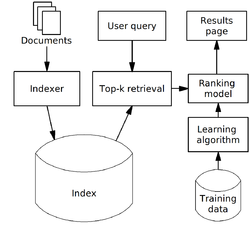
\includegraphics[scale=0.7]{./figures/letor.png}
\caption{An architecture of a machine-learned IR system from \protect\url{http://en.wikipedia.org/wiki/Learning_to_rank}} \label{fig:letor} 
\end{figure}
Figure~\ref{fig:letor} illustrates an architecture of a machine-learned IR system. How this architecture links to our approach will be discussed in
section~\ref{section:implementation}.

\subsection{Applying a Learned Model}\label{sec:background_applyLearnedModel}
Once a learned model has been generated, then for each document, the scores of each feature are multiplied by ones in the learned model and accumulated.
Finally, the accumulated scores for each document are sorted in descending order and documents with the high scores are ranked above
those with low scores.


\section{Tools}
This section will discussed tools used in this project. They are search engine platform Terrier, learning to rank library RankLib and evaluation tool,
trec\_eval.
\subsection{Terrier}\label{section:terrier} \hspace{0pt} \\
Every IR system requires programs that handle indexing, retrieving, ranking, etc. To build everything from scratch, it would be impossible within
the 1 year duration. However, there are a number of search engine platforms that deal with IR functionalities effectively.
Terrier~\cite{terrier} was chosen because it is a highly flexible, efficient, and effective open source search engine.
It is a comprehensive, and flexible platform for research and experimentation in text retrieval. Research can easily be 
carried out on standard TREC collection~\cite{trec}. 
Using Terrier, this project can easily extend from the existing search engine as it used Terrier as a search engine platform and it is written in Java
which is the same programming language used in this project.

\paragraph{Terrier Indexing}
\begin{figure}
\centering
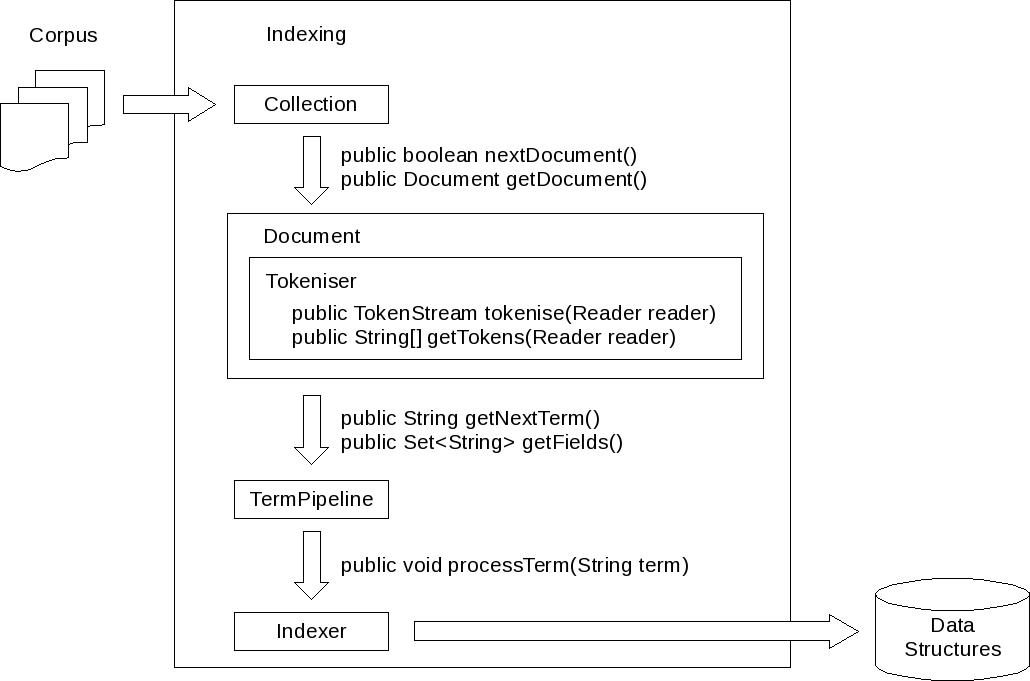
\includegraphics[scale=0.4]{./figures/terrierindexing.png}
\caption{Indexing Architecture of Terrier from \protect\url{http://terrier.org/docs/v3.5/basicComponents.html}} \label{fig:terrierindexing} 
\end{figure}

Figure~\ref{fig:terrierindexing} gives an overview of the interaction of the main components involved in the indexing process of Terrier.

\begin{quotation}
 \item 1. A corpus will be represented in the form of a \textbf{Collection} object. Raw text data will be represented in the form of a \textbf{Document} object. 
 Document implementations usually are provided with an instance of a \textbf{Tokeniser} class that breaks pieces of text into single indexing tokens.
 \item 2. The indexer is responsible for managing the indexing process. It iterates through the documents of the collection and sends each found 
 term through a \textbf{TermPipeline} component.
 \item 3. A TermPipeline can transform terms or remove terms that should not be indexed. An example for a TermPipeline chain is 
 termpipelines=Stopwords,PorterStemmer, which removes terms from the document using the \textbf{Stopwords} object, and then applies Porter's Stemming algorithm 
 for English to the terms.
 \item 4. Once terms have been processed through the TermPipeline, they are aggregated and the following data structures are created by their corresponding 
 DocumentBuilders: DirectIndex, DocumentIndex, Lexicon, and InvertedIndex.
 \item 5. For single-pass indexing, the structures are written in a different order. Inverted file postings are built in memory, and committed to 'runs' 
 when memory is exhausted. Once the collection had been indexed, all runs are merged to form the inverted index and the lexicon.
\end{quotation}

\subsection{RankLib}\label{section:rankLib}
RankLib~\cite{ranklib} is an open source library of learning to rank algorithms. It also implements many retrieval metrics to facilitate evaluation.
Currently eight popular algorithms have been implemented:
\begin{itemize}
 \item MART (Multiple Additive Regression Trees, a.k.a. Gradient boosted regression tree)
 \item RankNet
 \item RankBoost
 \item AdaRank
 \item Coordinate Ascent
 \item LambdaMART
 \item ListNet
 \item Random Forests
\end{itemize}

This library was chosen because it is easy to use, written in Java which can be easily combined with this system as it is also developed using Java, and
it implements 8 different learning to rank algorithms which makes it possible for users to try different algorithms.
However, AdaRank and Coordinate Ascent were only used in the project because other algorithms are too complex and not part of the scope of this project.

\subsection{trec\_eval}\label{sec:treceval}
trec\_eval is the standard tool used by the TREC community~\cite{trec} for evaluating a retrieval run, given the results file and a
standard set of judged results. trec\_eval was chosen because the data used in this project uses TREC format. 
It is easy to use and written in C which makes the tool efficient. To use trec\_eval, 2 files are required: qrels and result file in TREC format.
\textit{qrels} is a file that stores relevant results for queries stored in a queries file~\cite{qrels}. It has the following format~\cite{qrelsformat}:
\begin{quotation}
 \textit{TOPIC ITERATION DOCUMENT\# RELEVANCY}
\end{quotation}
where \textit{TOPIC} is the query, \textit{ITERATION} is the feedback iteration (almost always zero and not used),
\textit{DOCUMENT\#} is the official document number that corresponds to the "docno" field in the documents (in this project, expert's id), and
\textit{RELEVANCY} is a number indicating a degree of relevancy. In this project, 3 numbers: 0, 1, and 2 indicating non-relevant, relevant and perfectly
relevant respectively, are used. The result file is the file that contains the following~\cite{resultfileformat}:
\begin{quotation}
 \textit{TOPIC ITERATION DOCUMENT\# RANK SIM RUN\_ID}
\end{quotation}
where \textit{RANK} is the position of the corresponding document\# in a ranking, \textit{SIM} is a float value indicating a score and \textit{RUN\_ID}
is a string which gets printed out with the output.



\section{Expert Search}
In section~\ref{sec:expertsearch}, we discussed about the definition of Expert Search. This section will give 5 scenarios proposed by Yimam-Seid \& Kobsa
why expert search is needed~\cite[P. 387]{expertsearch}.
\begin{quotation}
  \item \textit{1. Access to non-documented information - e.g. in an organisation where not all relevant information is documented.}
  \item \textit{2. Specification need - the user is unable to formulate a plan to solve a problem, and resorts to seeking experts to assist them in formulating a plan.}
  \item \textit{3. Leveraging on another's expertise (group efficiency) - e.g. finding a piece of information that a relevant expert would know/find with
  less effort than the seeker.}
  \item \textit{4. Interpretation need - e.g. deriving the implications of, or understanding, a piece of information.}
  \item \textit{5. Socialisation need - the user may prefer that the human dimension be involved, as opposed to interacting with documents and computers.}
\end{quotation}

\subsection{Presenting Query Results}\label{sec:presentingQueryResult}
Figure~\ref{fig:retrieval_process} illustrates the process of search. From this figure, the process will start again if a user is not satisfied with 
the results. In this section, the focus is on how to convince user that a query result is good. Suppose a user who is currently studying software engineering
would like to know ``how to normalize database tables'', first of all, he needs to interpret his information need into a query which is ``database normalization''.
He then types his query into his preferred search engine. After he submits the query, the search engine gives him a list of results ranked by the degree
of relevancy. The question is how does he determine which result is what he is looking for?. Well, he could assume that the ranking provided by the search 
engine is correct. That is, the first result is what he is looking for. However, this is not always the case. He then explores each result and sees if 
it is the right one. But without exploring each result, could he be able to determine that which result is likely to satisfy his information need?
Perhaps, there has to be some evidence to convince him by just looking at the result. The followings are evidence he could take into account~\cite{craig}: 
\begin{itemize}
 \item URL
 \item Photo
 \item Author
 \item keywords of the article name
\end{itemize}
If a result in response to a query have all or some of these evidence, it has more credits than ones with no evidence at all. 
\begin{figure}
\centering
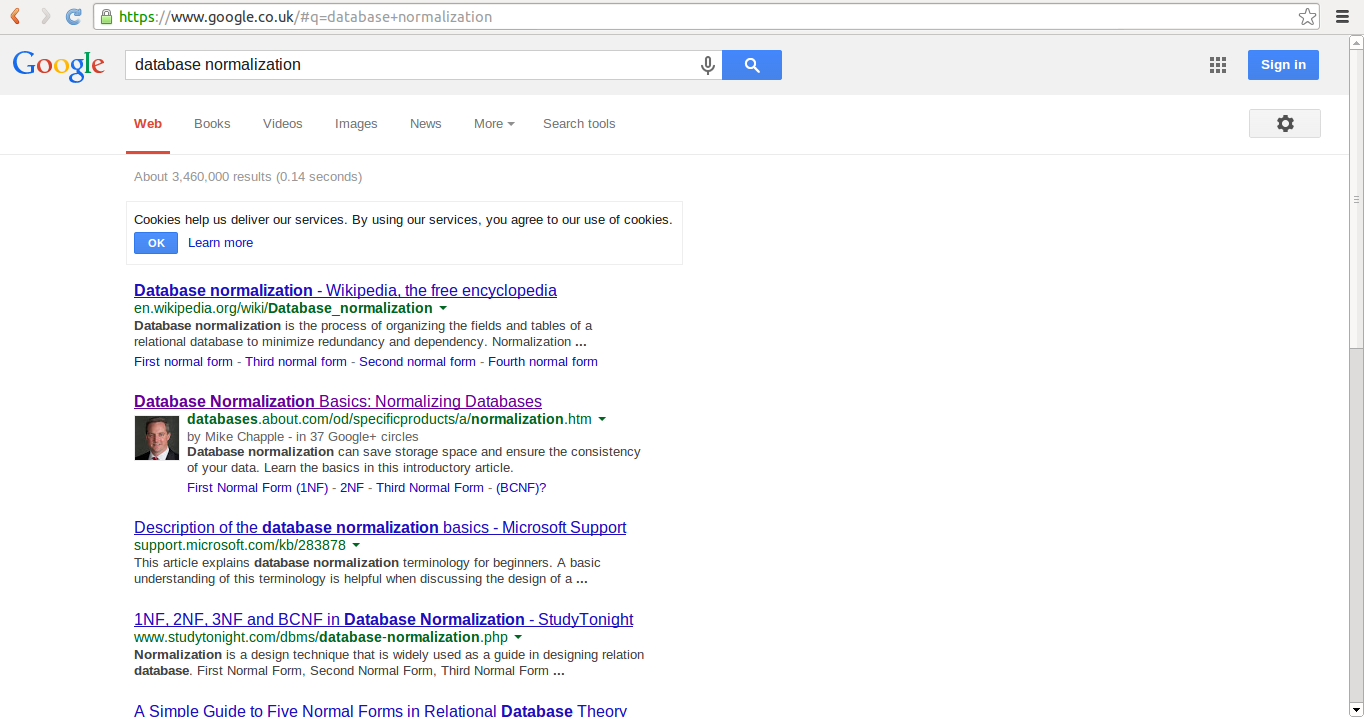
\includegraphics[scale=0.3]{./figures/query.png}
\caption{Sample Query} \label{fig:query}
\end{figure}
Figure \ref{fig:query} shows the results of the query ``database normalization''. It is obvious that from the top 4 results, all of the article names
include the keywords a user submitted, and the third result does not have query keywords included in the URL. Among all of which, the second result has more 
evidence than others. It has an author's name, a photo of an author that other results do not.

\subsection{Voting Technique}\label{section:voting}
In section ~\ref{section:retrieving}, we very briefly talked about weighting models or retrieval models. In other words, how documents are assigned scores. In this section,
it aims to give an overview of voting technique used in this project. To understand this section, readers must understand what data fusion technique is. 
``Data fustion techniques also known as metasearch techniques, are used to combine separate rankings of documents into a single ranking,
with the aim of improving over the performance of any constituent ranking''~\cite[P. 388]{expertsearch}. Within the context of this project, 
expert search is seen as a voting problem. The profile of each candidate is a set of documents associated to him to represent their expertise.
When each document associated to a candidate's profile get retrieved by the IR system, implicit vote for that candidate occurs~\cite[P. 389]{expertsearch}.
Data fusion technique is then used to combine the ranking with respect to the query and the implicit vote. In expert search task, it shows that 
``improving the quality of the underlying document representation can significantly improve the retrieval performance of the data fusion techniques 
on an expert search task''~\cite[P. 387]{expertsearch}. To give a simple example how data fusion technique works, take a look at this example

Let $R(Q)$ be the set of documents retrieved for query $Q$, and the set of documents belonging to the profile candidate $C$ be denoted $profile(C)$. In expert
search, we need to find a ranking of candidates, given $R(Q)$. Consider the simple example in Tables ~\ref{table:ranking} and ~\ref{table:profiles},
the ranking of documents with respect to the query has retrieved documents \{$D1, D2, D3, D4$\}. Using the candidate profiles, candidate $C1$ has accumulated
3 votes, $C2$ 2 votes, $C3$ 2 votes and $C4$ no votes. If all votes are counted equally, and each document in a candidate's profile is equally weighted, a possible
ranking of candidates to this query could be \{$C1, C2, C3$\}. In this project, the technique used is $expCombMNZ$ and the formula is as follows

\begin{table}
\centering
\begin{tabular}{|c|c|c|}
\hline \textbf{Rank} & \textbf{Docs} & \textbf{Scores}\\
\hline 1 & D1 & 5.4 \\
\hline 2 & D2 & 4.2\\
\hline 3 & D3 & 3.9 \\
\hline 4 & D4 & 2.0 \\  
\hline
\end{tabular}
\caption{R(Q)} \label{table:ranking}
\end{table}
\quad
\begin{table}
\centering
\begin{tabular}{|c|l|}
\hline \textbf{Profiles} & \textbf{Docs}\\
\hline C1 & D3, D4, D2 \\
\hline C2 & D1, D2 \\
\hline C3 & D3, D2 \\
\hline C4 & D5, D6 \\  
\hline
\end{tabular}
\caption{Profiles} \label{table:profiles}
\end{table}

\[
candScore(C,Q) = |R(Q) \cap profile(C)| \sum_{d \in R(Q) \cap profile(C)} exp(score_d)
\]
where $|R(Q) \cap profile(C)|$ is the number of documents from the profile of candidate $C$ that are in the ranking $R(Q)$ and $score_d$ is the score
obtained using retrieval model of candidate $C$.














